%!TEX root = /Users/stwaidele/Dropbox (Leisinger)/02 - AKAD/Projektbericht/Möglichkeiten der Digitalen Kontaktaufnahme im Endkundenbereich/vorlage.tex

\appendix
\section*{Anhang}
\addcontentsline{toc}{section}{Anhang}

\section*{Befragung der Kunden}
\label{sec:kundenbefragung}
\subsection*{Kundenfragebogen}
\addcontentsline{toc}{subsection}{Anhang 1: Kundenfragebogen}

Zur Datenerhebung wurde der auf den Seiten \pageref{pic:us1} bis \pageref{pic:us6} abgebildete Online–Fragebogen genutzt. 

\begin{figure}[H]
\begin{center}
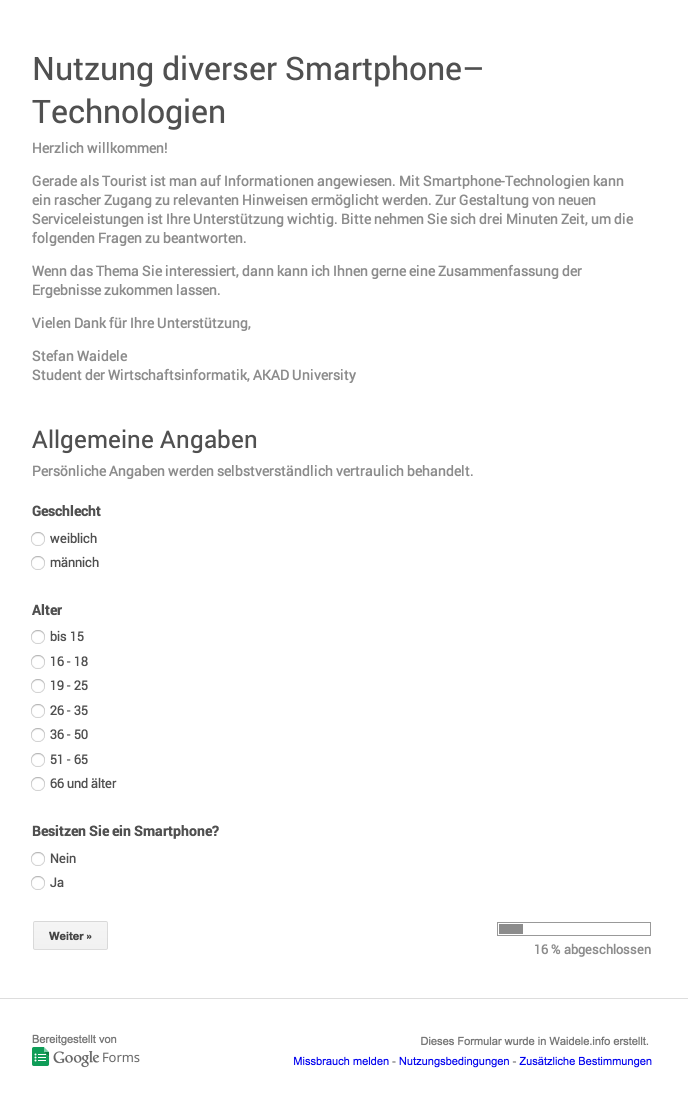
\includegraphics[width=.6\textwidth]{Umfrage-S1.png}
\caption{Screenshot: Umfrage Seite 1}
\label{pic:us1}
\end{center}
\end{figure}

\begin{figure}[H]
\begin{center}
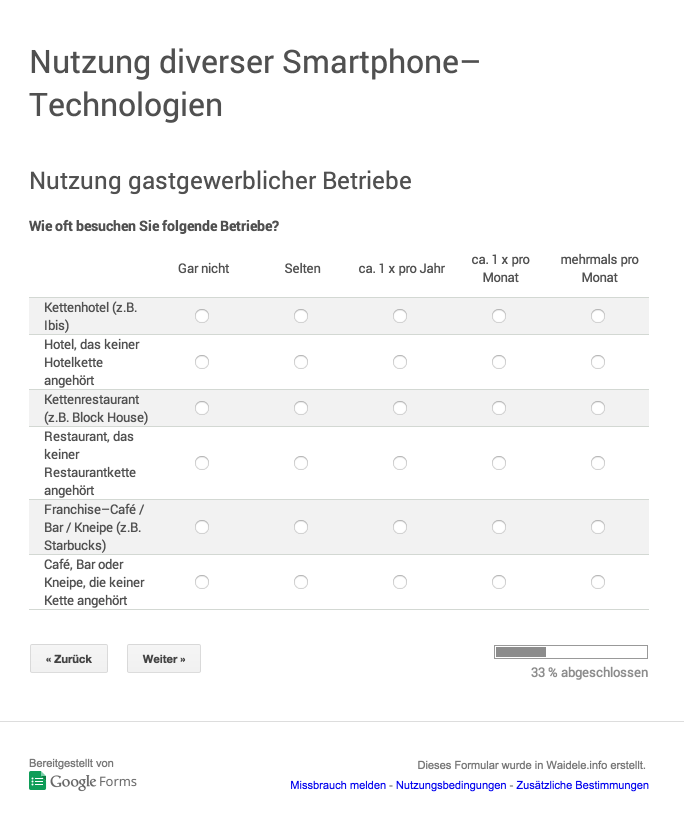
\includegraphics[width=.5\textwidth]{Umfrage-S2.png}
\caption{Screenshot: Umfrage Seite 2}
\label{pic:us2}
\end{center}
\end{figure}

\begin{figure}[H]
\begin{center}
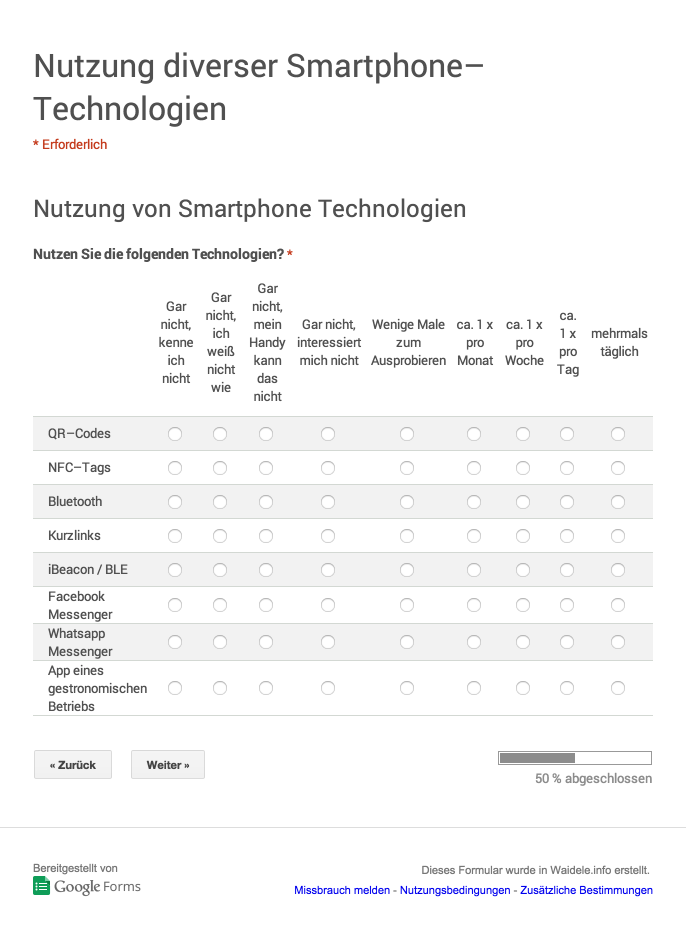
\includegraphics[width=.5\textwidth]{Umfrage-S3.png}
\caption{Screenshot: Umfrage Seite 3}
\label{pic:us3}
\end{center}
\end{figure}

\begin{figure}[H]
\begin{center}
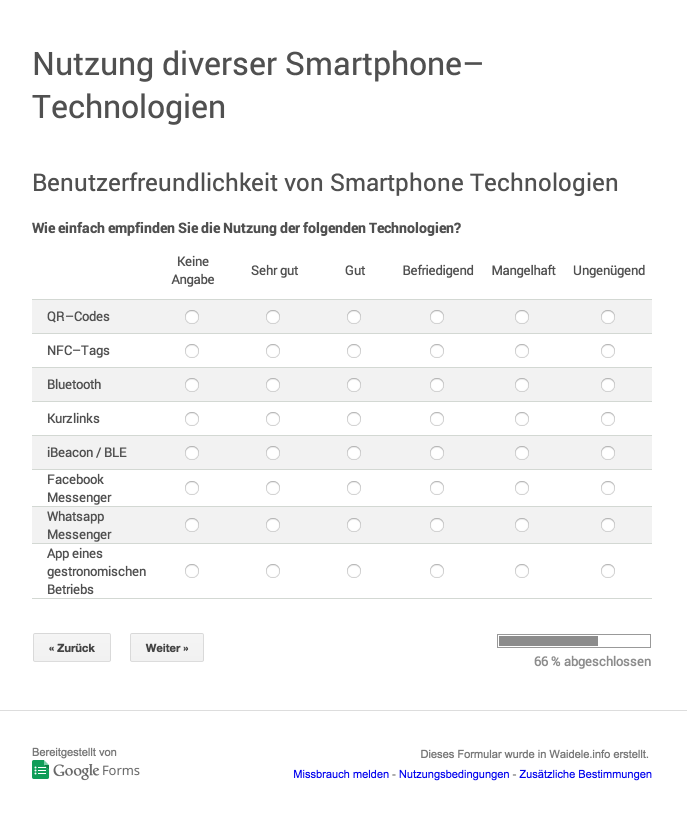
\includegraphics[width=.6\textwidth]{Umfrage-S4.png}
\caption{Screenshot: Umfrage Seite 4}
\label{pic:us4}
\end{center}
\end{figure}

\begin{figure}[H]
\begin{center}
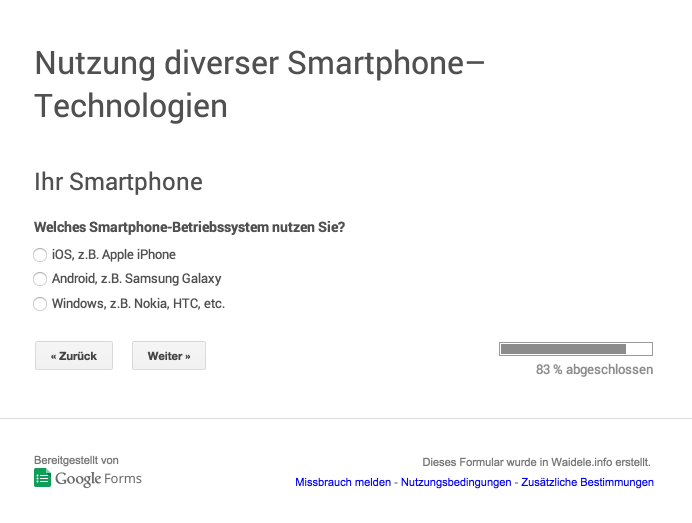
\includegraphics[width=.6\textwidth]{Umfrage-S5.png}
\caption{Screenshot: Umfrage Seite 5}
\label{pic:us5}
\end{center}
\end{figure}

\begin{figure}[H]
\begin{center}
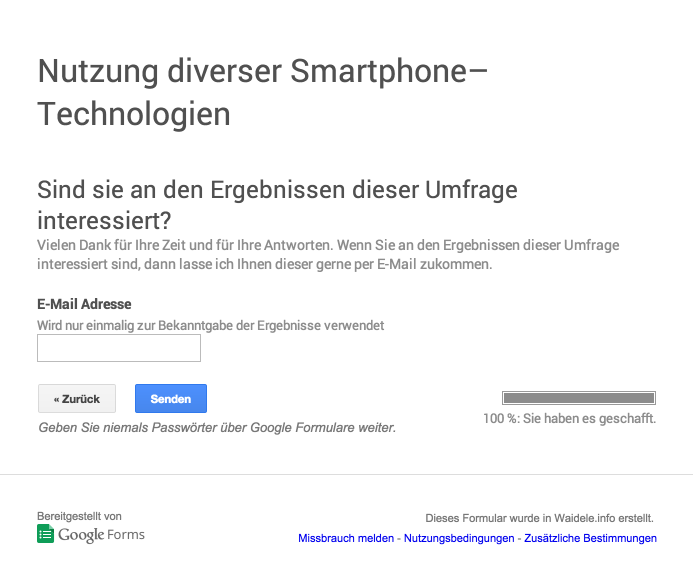
\includegraphics[width=.6\textwidth]{Umfrage-S6.png}
\caption{Screenshot: Umfrage Seite 6}
\label{pic:us6}
\end{center}
\end{figure}

\newpage
\subsection*{Anhang 2: Auswertung des Kundenfragebogens}
\addcontentsline{toc}{subsection}{Anhang 2: Auswertung des Kundenfragebogens}

Zwischen 12. August 2014 und 12. November 2014 wurden 174 Fragebögen ausgefüllt. 

Die Ergebnisse sind auf den Seiten \pageref{pic:aus1} bis \pageref{pic:aus4b} zusammengefasst. Differenzen zu 100\% entstehen durch Rundungsdifferenzen.

\begin{table}[H]
\begin{center}
\begin{footnotesize}
\begin{tabular}{| l | r  r |}  \hline                       
  \textbf{Geschlecht}              & \multicolumn{2}{|l|}{\textbf{Anzahl}}   \\ \hline 
  weiblich        &  109 &   (63\%)  \\  \hline  
  männlich        &  64  &   (37\%)  \\  \hline  
  keine Angabe    &  1   &   (1\%)  \\  \hline  
  \textbf{Summe}  & 174  &   \\  \hline  
\end{tabular}
\end{footnotesize}
\caption{Umfrageauswertung: Geschlecht}
\label{tab:geschlecht}
\end{center}
\end{table}

\begin{table}[H]
\begin{center}
\begin{footnotesize}
\begin{tabular}{| l | r  r |}  \hline                       
  \textbf{Altersklasse}              & \multicolumn{2}{|l|}{\textbf{Anzahl}}   \\ \hline 
  bis 15          &  0 &   (0\%)  \\  \hline  
  16 bis 18       &  1 &   (<1\%)  \\  \hline  
  19 bis 25       & 20  &   (11\%)  \\  \hline  
  26 bis 35       & 95  &   (55\%)  \\  \hline  
  36 bis 50       & 42  &   (24\%)  \\  \hline  
  51 bis 65       & 16  &   (9\%)  \\  \hline  
  66 und älter    & 0  &   (0\%)  \\  \hline  
  \textbf{Summe}  & 174  &   \\  \hline  
\end{tabular}
\end{footnotesize}
\caption{Umfrageauswertung: Altersklassen}
\label{tab:altersklassen}
\end{center}
\end{table}

\begin{table}[H]
\begin{center}
\begin{footnotesize}
\begin{tabular}{| l | r  r |}  \hline                       
  \textbf{Smartphone}              & \multicolumn{2}{|l|}{\textbf{Anzahl}}   \\ \hline 
  ja        &  161 &   (93\%)  \\  \hline  
  nein        &  12  &   (7\%)  \\  \hline  
  keine Angabe    &  1   &   (<1\%)  \\  \hline  
  \textbf{Summe}  & 174  &   \\  \hline  
\end{tabular}
\end{footnotesize}
\caption{Umfrageauswertung: Smartphone}
\label{tab:smartphone}
\end{center}
\end{table}

\begin{table}[H]
\begin{center}
\begin{footnotesize}
\begin{tabular}{| l | r  r |}  \hline                       
  \textbf{Smartphone}              & \multicolumn{2}{|l|}{\textbf{Anzahl}}   \\ \hline 
  Android    &  83 &   (50\%)  \\  \hline  
  iOS        &  71  &   (43\%)  \\  \hline  
  Windows    &  7   &   (7\%)  \\  \hline  
  \textbf{Summe}  & 166  &   \\  \hline  
\end{tabular}
\end{footnotesize}
\caption{Umfrageauswertung: Betriebssysteme}
\label{tab:smartphone}
\end{center}
\end{table}

\begin{table}[H]
\begin{center}
\begin{footnotesize}
\begin{tabular}{| l | C{1cm} | C{1cm} | C{1cm} | C{1cm} | C{1cm} |}  \hline
  \textbf{Frequenz} & 
	\begin{turn}{90}\textbf{Gar nicht}\end{turn} & 
	\begin{turn}{90}\textbf{Selten}\end{turn}  & 
	\begin{turn}{90}\textbf{ca. 1 x pro Jahr}\end{turn} & 
	\begin{turn}{90}\textbf{ca. 1 x pro Monat}\end{turn} & 
	\begin{turn}{90}\textbf{mehrmals monatlich}\end{turn}\\ \hline 
	\multirow{2}{*}{Kettenhotel}  & 27 & 59 & 59 & 23 & 6\\  
		                          & (16\%) & (34\%) & (34\%) & (13\%) & (3\%) \\  \hline  
	\multirow{2}{*}{Individualhotel} & 13 & 67 & 76 & 16 & 2\\   
		                             & (7\%) & (39\%) & (44\%) & (9\%) & (1\%) \\  \hline  
	\multirow{2}{*}{Kettenrestaurant} 	 & 26 & 48  & 57  & 38   & 5\\  
		      & (15\%) & (28\%) & (33\%) & (22\%) & (3\%) \\  \hline  
	\multirow{2}{*}{Individualrestaurant} &  8  & 20   & 30  & 86   & 30\\   
		      & (5\%) & (11\%) & (17\%) & (49\%) & (17\%) \\  \hline  
	\multirow{2}{*}{Kettencafé} &  24  &  55  & 38  & 42   & 15\\  
		      & (14\%) & (32\%) & (22\%) & (24\%) & (7\%) \\  \hline  
	\multirow{2}{*}{Individualcafé} & 7   &  24  & 18  & 77   & 48\\   
		      & (4\%) & (14\%) & (10\%) & (44\%) & (28\%) \\  \hline  
\end{tabular}
\end{footnotesize}
\caption{Umfrageauswertung: Nutzung gastgewerblicher Betriebe}
\label{tab:gastronutzung}
\end{center}
\end{table}


\begin{table}[H]
\begin{center}
\begin{footnotesize}
\begin{tabular}{| l | C{1cm} | C{1cm} | C{1cm} | C{1cm} | C{1cm} | C{1cm} | C{1cm} | C{1cm} | C{1cm} |}  \hline
  \textbf{Technologie} & 
	\begin{turn}{90}\textbf{Gar nicht, …}\end{turn} & 
	\begin{turn}{90}\textbf{Wenige male zum Ausprobieren}\end{turn}  & 
	\begin{turn}{90}\textbf{ca. 1 x pro Monat}\end{turn} & 
	\begin{turn}{90}\textbf{ca. 1 x pro Woche}\end{turn} & 
	\begin{turn}{90}\textbf{ca. 1 x am Tag}\end{turn} & 
	\begin{turn}{90}\textbf{mehrmals täglich}\end{turn}\\ \hline 
	\multirow{2}{*}{QR Codes}   &  62    &  82    &  22    &  8   &  \multirow{2}{*}{—}    & \multirow{2}{*}{—}    \\  
		                       & (36\%) & (47\%) & (13\%) & (5\%) &  &  \\  \hline  
	\multirow{2}{*}{NFC Tags}   &  142    &  26    &  4    &  2   &  \multirow{2}{*}{—}    & \multirow{2}{*}{—}    \\  
		                       & (82\%) & (15\%) & (2\%) & (1\%) &  &  \\  \hline  
	\multirow{2}{*}{Bluetooth}    &  34    & 35     & 37     & 23    & 17     & 28    \\  
		                       & (20\%)    & (20\%) & (21\%) & (13\%) & (10\%) & (16\%) \\  \hline  
	\multirow{2}{*}{Kurzlinks}    & 70     &  23    & 29     & 21    &  12    & 19    \\  
		                          & (40\%) & (13\%) & (17\%) & (12\%) & (7\%) & (11\%) \\  \hline  
	\multirow{2}{*}{iBeacon / BLE}    & 161     & 11     &   \multirow{2}{*}{—}    &  \multirow{2}{*}{—}    &  2    &  \multirow{2}{*}{—}    \\  
		                              & (93\%) & (6\%) &  &  & (1\%) &  \\  \hline  
	\multirow{2}{*}{Facebook Messenger}    &      &      &      &     &      &     \\  
		                                   & (\%) & (\%) & (\%) & (\%) & (\%) & (\%) \\  \hline  
	\multirow{2}{*}{Whatsapp Messenger}    &      &      &      &     &      &     \\  
		                                   & (\%) & (\%) & (\%) & (\%) & (\%) & (\%) \\  \hline  
	\multirow{2}{*}{App eines Betriebes}   &      &      &      &     &      &     \\  
		                                   & (\%) & (\%) & (\%) & (\%) & (\%) & (\%) \\  \hline  
\end{tabular}
\end{footnotesize}
\caption{Umfrageauswertung: Nutzung von Smartphone Technologien}
\label{tab:gastronutzung}
\end{center}
\end{table}

\begin{table}[H]
\begin{center}
\begin{footnotesize}
\begin{tabular}{| l | C{1cm} | C{1cm} | C{1cm} | C{1cm} |}  \hline
  \textbf{Technologie} & 
	\begin{turn}{90}\textbf{Gar nicht, kenne ich nicht}\end{turn} & 
	\begin{turn}{90}\textbf{Gar nicht, ich weiß nicht wie}\end{turn} & 
	\begin{turn}{90}\textbf{Gar nicht, mein Handy kann das nicht}\end{turn} & 
	\begin{turn}{90}\textbf{Gar nicht, interessiert mich nicht}\end{turn} \\ \hline 
	\multirow{2}{*}{QR Codes}  &  28    & 26     & 2     & 6     \\  
		                       & (16\%) & (15\%) & (1\%) & (3\%) \\  \hline  
	\multirow{2}{*}{NFC Tags}  &  38    & 72     & 5     &  27    \\  
		                       & (22\%) & (41\%) & (3\%) & (16\%) \\  \hline  
	\multirow{2}{*}{Bluetooth}  &  22    & 7     & 2     & 3     \\  
		                       & (13\%) & (4\%) & (1\%) & (2\%) \\  \hline  
	\multirow{2}{*}{Kurzlinks}   & 28     & 35     & 2     & 5     \\  
		                         & (16\%) & (20\%) & (1\%) & (3\%) \\  \hline  
	\multirow{2}{*}{iBeacon / BLE}   &  28    & 117     & 6     & 10     \\  
		                       & (16\%) & (67\%) & (3\%) & (6\%) \\  \hline  
	\multirow{2}{*}{Facebook Messenger}   &      &      &      &      \\  
		                       & (\%) & (\%) & (\%) & (\%) \\  \hline  
	\multirow{2}{*}{Whatsapp Messenger}   &      &      &      &      \\  
		                       & (\%) & (\%) & (\%) & (\%) \\  \hline  
	\multirow{2}{*}{App eines Betriebes}   &      &      &      &      \\  
		                       & (\%) & (\%) & (\%) & (\%) \\  \hline  
\end{tabular}
\end{footnotesize}
\caption{Umfrageauswertung: Gründe für die Nicht–Nutzung}
\label{tab:gastronutzung}
\end{center}
\end{table}

\begin{table}[H]
\begin{center}
\begin{footnotesize}
\begin{tabular}{| l | C{1cm} | C{1cm} | C{1cm} | C{1cm} | C{1cm} | C{1cm} | C{1cm} | C{1cm} | C{1cm} |}  \hline
  \textbf{Technologie} & 
	\begin{turn}{90}\textbf{Keine Angabe}\end{turn} & 
	\begin{turn}{90}\textbf{Sehr gut}\end{turn}  & 
	\begin{turn}{90}\textbf{Gut}\end{turn} & 
	\begin{turn}{90}\textbf{Befriedigend}\end{turn} & 
	\begin{turn}{90}\textbf{Mangelhaft}\end{turn} & 
	\begin{turn}{90}\textbf{Ausreichend}\end{turn}\\ \hline 
	\multirow{2}{*}{QR Codes}   &      &      &      &     &      &     \\  
		                       & (\%) & (\%) & (\%) & (\%) & (\%) & (\%) \\  \hline  
	\multirow{2}{*}{NFC Tags}   &      &      &      &     &      &     \\  
		                       & (\%) & (\%) & (\%) & (\%) & (\%) & (\%) \\  \hline  
	\multirow{2}{*}{Bluetooth}    &      &      &      &     &      &     \\  
		                       & (\%) & (\%) & (\%) & (\%) & (\%) & (\%) \\  \hline  
	\multirow{2}{*}{Kurzlinks}    &      &      &      &     &      &     \\  
		                       & (\%) & (\%) & (\%) & (\%) & (\%) & (\%) \\  \hline  
	\multirow{2}{*}{iBeacon / BLE}    &      &      &      &     &      &     \\  
		                       & (\%) & (\%) & (\%) & (\%) & (\%) & (\%) \\  \hline  
	\multirow{2}{*}{Facebook Messenger}    &      &      &      &     &      &     \\  
		                       & (\%) & (\%) & (\%) & (\%) & (\%) & (\%) \\  \hline  
	\multirow{2}{*}{Whatsapp Messenger}    &      &      &      &     &      &     \\  
		                       & (\%) & (\%) & (\%) & (\%) & (\%) & (\%) \\  \hline  
	\multirow{2}{*}{App eines Betriebes}    &      &      &      &     &      &     \\  
		                       & (\%) & (\%) & (\%) & (\%) & (\%) & (\%) \\  \hline  
\end{tabular}
\end{footnotesize}
\caption{Umfrageauswertung: Benutzerfreundlichkeit von Smartphone Technologien}
\label{tab:gastronutzung}
\end{center}
\end{table}
